\documentclass{article}
\usepackage[final]{nips_2018}
\usepackage[utf8]{inputenc}
\usepackage[T1]{fontenc}

\usepackage{hyperref}
\usepackage{url}
\usepackage{booktabs}
\usepackage{amsfonts}
\usepackage{nicefrac}
\usepackage{enumerate}
\usepackage{microtype}
\usepackage{graphicx}
\usepackage{amsmath}
\usepackage{amsthm}
\usepackage{caption}
\usepackage{multirow}
\usepackage{enumitem}

\renewcommand{\thesubsubsection}{\thesubsection\,\alph{subsubsection})}
\newcommand{\del}[2]{\ensuremath{\frac{\partial #1}{\partial #2}}}
\newcommand{\Ell}{\ensuremath{\mathcal{L}}}

\title{Assignment 2\\Recurrent Neural Networks and Graph Neural Networks}

\author{
  Francesco Dal Canton \\
  \texttt{f.dal.canton@student.uva.nl} \\
  12404225
}

\begin{document}

\maketitle

%################################# NEW SECTION ##################################
\section{Vanilla RNN versus LSTM}

%###################### NEW SUBSECTION #######################
\subsection{Toy Problem: Palindrome Numbers}

%###################### NEW SUBSECTION #######################
\subsection{Vanilla RNN in PyTorch}

\begin{enumerate}[label=\textbf{1.\arabic*}]
  \item
  Throughout this assignment I use the notation $x_T$ in place of $x^{(T)}$ used in the assignment text. I also make the choice to ignore the $tanh$ function, which would only appear as an additional $\partial$-term in each application of the chain rule.

  That said, we can easily write the expression for the gradient of the loss w.r.t. the output weights as follows.

  \begin{align*}
    \del{\Ell_T}{W_{ph}} &= \del{\Ell_T}{\hat{y}_T} \del{\hat{y}_T}{p_T} \del{p_T}{W_{ph}} \\
    &= \del{\Ell_T}{\hat{y}_T} \del{\hat{y}_T}{p_T} h_T^T
  \end{align*}

  Defining the gradient w.r.t the hidden weights is trickier. We can start by writing out the standard chain rule formulation, which we can compress by omitting parts that we've defined in the previous assignment (i.e. cross-entropy, softmax, etc.).

  \begin{align*}
    \del{\Ell_T}{W_{hh}} &= \del{\Ell_T}{\hat{y}_T} \del{\hat{y}_T}{p_T} \del{p_T}{h_T} \del{h_T}{W_{hh}} \\
    &= \del{\Ell_T}{h_T} \del{h_T}{W_{hh}}
  \end{align*}

  We notice that any $h_t$ depends recursively on $h_{t-1}$ which itself depends on $W_{hh}$. We can then define the gradient of the last hidden state w.r.t. its weights, and develop it using the product rule.

  \begin{align*}
    \del{h_T}{W_{hh}} &= \del{\left[ W_{hx} x_T + W_{hh} h_{T-1} + b_h \right]}{W_{hh}} \\
    &= \del{\left[ W_{hh} h_{T-1} \right]}{W_{hh}} \\
    &= \del{W_{hh}}{W_{hh}} h_{T-1} + W_{hh} \del{h_{T-1}}{W_{hh}} \\
    &= h_{T-1} + W_{hh} \del{h_{T-1}}{W_{hh}}
  \end{align*}

  Where, at the end of the recursive chain, we reach the gradient of $h_0$ w.r.t. the hidden weights, which is $0$. With this knowledge, we can expand the chain in order to compress it again.

  \begin{align*}
    \del{h_T}{W_{hh}} &= h_{T-1} + W_{hh} \left( h_{T-2} + W_{hh} \left( h_{T-3} + W_{hh} \left( \dots \right) \right) \right) \\
    &= h_{T-1} + W_{hh} h_{T-2} + W_{hh}^2 h_{T-3} + \dots + W_{hh}^{T-2} h_{T-(T-1)} \\
    &= \sum_{i=1}^{T-1} W_{hh}^{i-1} h_{T-i}
  \end{align*}

  So that we can express the original gradient as:

  \begin{align*}
    \del{\Ell_T}{W_{hh}} &= \del{\Ell_T}{h_T} \sum_{i=1}^{T-1} W_{hh}^{i-1} h_{T-i}
  \end{align*}

  The most striking difference between the gradient of the loss w.r.t. the output weights and the one w.r.t. the hidden weights is that the latter involves a temporal dependency that extends all the way to the first time step of the cell's operation. In other words, after feeding the RNN a sequence of $n$ inputs, in order to perform backpropagation we need to multiply the gradient by the hidden weight matrix a large number of times, which grows exponentially with the number of time steps.

  This fact causes the well known problem of vanishing or exploding gradients. When performing an update over a large number of timesteps, the gradient that should pertain to the gradients further back in time either reduces to $0$ or it increases to infinity, depending on whether the hidden weights are small or large. This makes it very hard to train such networks for long sequences, since those longer time dependencies can't be learned.

  \item
  \item
  \item
\end{enumerate}

%###################### NEW SUBSECTION #######################
\subsection{Long-Short Term Network (LSTM) in PyTorch}

\begin{enumerate}[label=\textbf{1.\arabic*}]
  \setcounter{enumi}{4}
  \item

  \begin{enumerate}[label=\textbf{(\alph*)}]
    \item
    \item
  \end{enumerate}

  \item
\end{enumerate}

%################################# NEW SECTION ##################################
\section{Recurrent Nets as Generative Model}

\begin{enumerate}[label=\textbf{2.\arabic*}]
  \item

  \begin{enumerate}[label=\textbf{(\alph*)}]
    \item
    \item
    \item
  \end{enumerate}

  \item
\end{enumerate}

%################################# NEW SECTION ##################################
\section{Graph Neural Networks}

%###################### NEW SUBSECTION #######################
\subsection{GCN Forward Layer}

\begin{enumerate}[label=\textbf{3.\arabic*}]
  \item

  \begin{enumerate}[label=\textbf{(\alph*)}]
    \item
    \item
  \end{enumerate}
\end{enumerate}

%###################### NEW SUBSECTION #######################
\subsection{Applications of GNNs}

\begin{enumerate}[label=\textbf{3.\arabic*}]
  \setcounter{enumi}{1}
  \item
\end{enumerate}

%###################### NEW SUBSECTION #######################
\subsection{Comparing and Combining GNNs and RNNs}

\begin{enumerate}[label=\textbf{3.\arabic*}]
  \setcounter{enumi}{2}
  \item

  \begin{enumerate}[label=\textbf{(\alph*)}]
    \item
    \item
  \end{enumerate}
\end{enumerate}

% \begin{figure}[h]
%     \centering
%     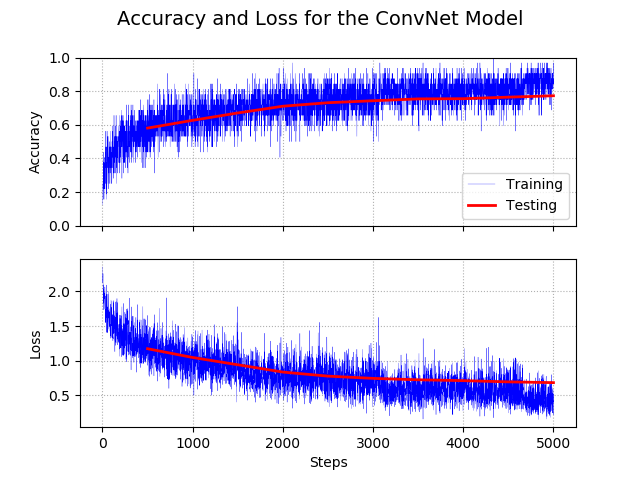
\includegraphics[scale=0.7]{img/convnet_results.png}
%     \caption{Training and test accuracies and losses for the ConvNet model. The test accuracies and losses are produced every 500 steps. The final test accuracy was $77.3\%$}
%     \label{fig:convnet_results}
% \end{figure}


\end{document}
